\documentclass[twoside]{book}

% Packages required by doxygen
\usepackage{fixltx2e}
\usepackage{calc}
\usepackage{doxygen}
\usepackage[export]{adjustbox} % also loads graphicx
\usepackage{graphicx}
\usepackage[utf8]{inputenc}
\usepackage{makeidx}
\usepackage{multicol}
\usepackage{multirow}
\PassOptionsToPackage{warn}{textcomp}
\usepackage{textcomp}
\usepackage[nointegrals]{wasysym}
\usepackage[table]{xcolor}

% Font selection
\usepackage[T1]{fontenc}
\usepackage[scaled=.90]{helvet}
\usepackage{courier}
\usepackage{amssymb}
\usepackage{sectsty}
\renewcommand{\familydefault}{\sfdefault}
\allsectionsfont{%
  \fontseries{bc}\selectfont%
  \color{darkgray}%
}
\renewcommand{\DoxyLabelFont}{%
  \fontseries{bc}\selectfont%
  \color{darkgray}%
}
\newcommand{\+}{\discretionary{\mbox{\scriptsize$\hookleftarrow$}}{}{}}

% Page & text layout
\usepackage{geometry}
\geometry{%
  a4paper,%
  top=2.5cm,%
  bottom=2.5cm,%
  left=2.5cm,%
  right=2.5cm%
}
\tolerance=750
\hfuzz=15pt
\hbadness=750
\setlength{\emergencystretch}{15pt}
\setlength{\parindent}{0cm}
\setlength{\parskip}{3ex plus 2ex minus 2ex}
\makeatletter
\renewcommand{\paragraph}{%
  \@startsection{paragraph}{4}{0ex}{-1.0ex}{1.0ex}{%
    \normalfont\normalsize\bfseries\SS@parafont%
  }%
}
\renewcommand{\subparagraph}{%
  \@startsection{subparagraph}{5}{0ex}{-1.0ex}{1.0ex}{%
    \normalfont\normalsize\bfseries\SS@subparafont%
  }%
}
\makeatother

% Headers & footers
\usepackage{fancyhdr}
\pagestyle{fancyplain}
\fancyhead[LE]{\fancyplain{}{\bfseries\thepage}}
\fancyhead[CE]{\fancyplain{}{}}
\fancyhead[RE]{\fancyplain{}{\bfseries\leftmark}}
\fancyhead[LO]{\fancyplain{}{\bfseries\rightmark}}
\fancyhead[CO]{\fancyplain{}{}}
\fancyhead[RO]{\fancyplain{}{\bfseries\thepage}}
\fancyfoot[LE]{\fancyplain{}{}}
\fancyfoot[CE]{\fancyplain{}{}}
\fancyfoot[RE]{\fancyplain{}{\bfseries\scriptsize Generated by Doxygen }}
\fancyfoot[LO]{\fancyplain{}{\bfseries\scriptsize Generated by Doxygen }}
\fancyfoot[CO]{\fancyplain{}{}}
\fancyfoot[RO]{\fancyplain{}{}}
\renewcommand{\footrulewidth}{0.4pt}
\renewcommand{\chaptermark}[1]{%
  \markboth{#1}{}%
}
\renewcommand{\sectionmark}[1]{%
  \markright{\thesection\ #1}%
}

% Indices & bibliography
\usepackage{natbib}
\usepackage[titles]{tocloft}
\setcounter{tocdepth}{3}
\setcounter{secnumdepth}{5}
\makeindex

% Hyperlinks (required, but should be loaded last)
\usepackage{ifpdf}
\ifpdf
  \usepackage[pdftex,pagebackref=true]{hyperref}
\else
  \usepackage[ps2pdf,pagebackref=true]{hyperref}
\fi
\hypersetup{%
  colorlinks=true,%
  linkcolor=blue,%
  citecolor=blue,%
  unicode%
}

% Custom commands
\newcommand{\clearemptydoublepage}{%
  \newpage{\pagestyle{empty}\cleardoublepage}%
}

\usepackage{caption}
\captionsetup{labelsep=space,justification=centering,font={bf},singlelinecheck=off,skip=4pt,position=top}

%===== C O N T E N T S =====

\begin{document}

% Titlepage & ToC
\hypersetup{pageanchor=false,
             bookmarksnumbered=true,
             pdfencoding=unicode
            }
\pagenumbering{roman}
\begin{titlepage}
\vspace*{7cm}
\begin{center}%
{\Large Holonomic Control }\\
\vspace*{1cm}
{\large Generated by Doxygen 1.8.11}\\
\end{center}
\end{titlepage}
\clearemptydoublepage
\tableofcontents
\clearemptydoublepage
\pagenumbering{arabic}
\hypersetup{pageanchor=true}

%--- Begin generated contents ---
\chapter{File Index}
\section{File List}
Here is a list of all files with brief descriptions\+:\begin{DoxyCompactList}
\item\contentsline{section}{\hyperlink{holo__movement_8cpp}{holo\+\_\+movement.\+cpp} }{\pageref{holo__movement_8cpp}}{}
\item\contentsline{section}{\hyperlink{random__position__server_8cpp}{random\+\_\+position\+\_\+server.\+cpp} }{\pageref{random__position__server_8cpp}}{}
\item\contentsline{section}{\hyperlink{target__velocity__server_8cpp}{target\+\_\+velocity\+\_\+server.\+cpp} }{\pageref{target__velocity__server_8cpp}}{}
\end{DoxyCompactList}

\chapter{File Documentation}
\hypertarget{holo__movement_8cpp}{}\section{holo\+\_\+movement.\+cpp File Reference}
\label{holo__movement_8cpp}\index{holo\+\_\+movement.\+cpp@{holo\+\_\+movement.\+cpp}}
{\ttfamily \#include \char`\"{}ros/ros.\+h\char`\"{}}\\*
{\ttfamily \#include \char`\"{}geometry\+\_\+msgs/\+Twist.\+h\char`\"{}}\\*
{\ttfamily \#include \char`\"{}nav\+\_\+msgs/\+Odometry.\+h\char`\"{}}\\*
{\ttfamily \#include \char`\"{}holo\+\_\+control/\+Target\+Pos.\+h\char`\"{}}\\*
{\ttfamily \#include \char`\"{}holo\+\_\+control/\+Target\+Vel.\+h\char`\"{}}\\*
{\ttfamily \#include $<$sstream$>$}\\*
{\ttfamily \#include $<$iostream$>$}\\*
{\ttfamily \#include $<$math.\+h$>$}\\*
Include dependency graph for holo\+\_\+movement.\+cpp\+:\nopagebreak
\begin{figure}[H]
\begin{center}
\leavevmode
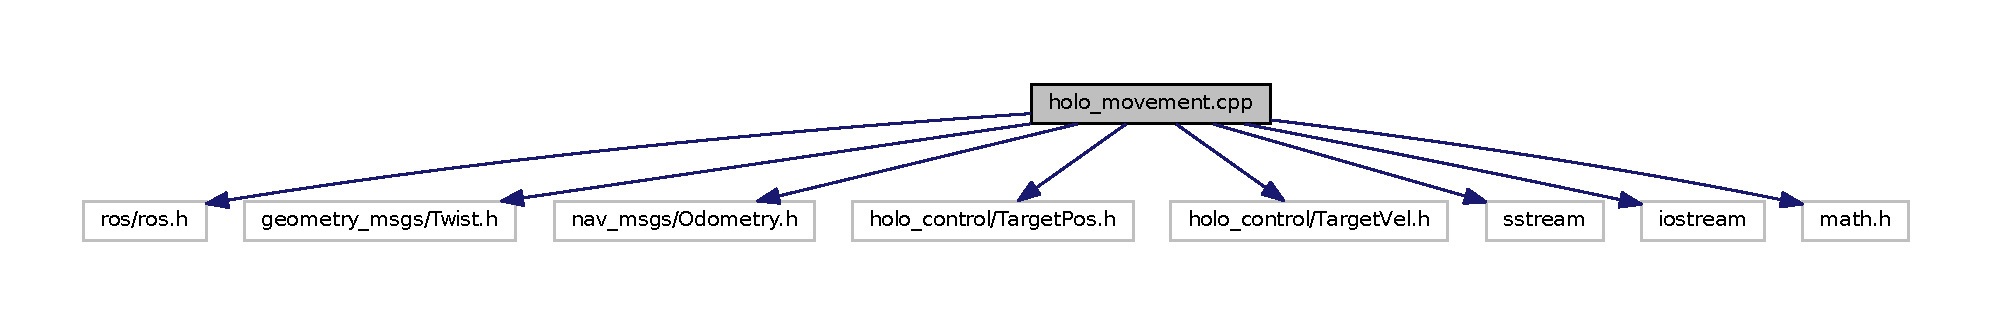
\includegraphics[width=350pt]{holo__movement_8cpp__incl}
\end{center}
\end{figure}
\subsection*{Functions}
\begin{DoxyCompactItemize}
\item 
float \hyperlink{holo__movement_8cpp_aaf85da3833058c8adfd6b67cf0b36885}{norm2} (float x, float y, float tx, float ty)
\item 
void \hyperlink{holo__movement_8cpp_aef70658f8ec02213922917e67d9e1c76}{subscriber\+Callback} (const nav\+\_\+msgs\+::\+Odometry\+::\+Const\+Ptr \&pose\+\_\+msg)
\item 
int \hyperlink{holo__movement_8cpp_a3c04138a5bfe5d72780bb7e82a18e627}{main} (int argc, char $\ast$$\ast$argv)
\end{DoxyCompactItemize}
\subsection*{Variables}
\begin{DoxyCompactItemize}
\item 
ros\+::\+Publisher \hyperlink{holo__movement_8cpp_a350594df3e8f6948c8462edfd41ce086}{pub}
\item 
ros\+::\+Service\+Client \hyperlink{holo__movement_8cpp_a9a132f5e7094e7dfbb0283cd6865552a}{client\+\_\+target}
\item 
ros\+::\+Service\+Client \hyperlink{holo__movement_8cpp_aa9a414283399446e6bf92415ebdac48e}{client\+\_\+vel}
\item 
geometry\+\_\+msgs\+::\+Point \hyperlink{holo__movement_8cpp_a856d701335ffc8b8bad1223902b1a009}{target\+\_\+pos}
\item 
float \hyperlink{holo__movement_8cpp_a7bf48396f7b1614eacfc04b4a25f434e}{dist\+\_\+th} = 0.\+1
\item 
int \hyperlink{holo__movement_8cpp_ac0c4717781a654470cef2abd04e7c1e2}{vel\+\_\+algorithm} = 0
\end{DoxyCompactItemize}


\subsection{Function Documentation}
\index{holo\+\_\+movement.\+cpp@{holo\+\_\+movement.\+cpp}!main@{main}}
\index{main@{main}!holo\+\_\+movement.\+cpp@{holo\+\_\+movement.\+cpp}}
\subsubsection[{\texorpdfstring{main(int argc, char $\ast$$\ast$argv)}{main(int argc, char **argv)}}]{\setlength{\rightskip}{0pt plus 5cm}int main (
\begin{DoxyParamCaption}
\item[{int}]{argc, }
\item[{char $\ast$$\ast$}]{argv}
\end{DoxyParamCaption}
)}\hypertarget{holo__movement_8cpp_a3c04138a5bfe5d72780bb7e82a18e627}{}\label{holo__movement_8cpp_a3c04138a5bfe5d72780bb7e82a18e627}


Definition at line 109 of file holo\+\_\+movement.\+cpp.

\index{holo\+\_\+movement.\+cpp@{holo\+\_\+movement.\+cpp}!norm2@{norm2}}
\index{norm2@{norm2}!holo\+\_\+movement.\+cpp@{holo\+\_\+movement.\+cpp}}
\subsubsection[{\texorpdfstring{norm2(float x, float y, float tx, float ty)}{norm2(float x, float y, float tx, float ty)}}]{\setlength{\rightskip}{0pt plus 5cm}float norm2 (
\begin{DoxyParamCaption}
\item[{float}]{x, }
\item[{float}]{y, }
\item[{float}]{tx, }
\item[{float}]{ty}
\end{DoxyParamCaption}
)}\hypertarget{holo__movement_8cpp_aaf85da3833058c8adfd6b67cf0b36885}{}\label{holo__movement_8cpp_aaf85da3833058c8adfd6b67cf0b36885}
Function to compute norm of vector

This function computes the euclidean norm of the vector identified by starting and ending points passed as arguments


\begin{DoxyParams}{Parameters}
{\em x} & (float)\+: starting point X coordinate; \\
\hline
{\em y} & (float)\+: starting point Y coordinate; \\
\hline
{\em tx} & (float)\+: ending point X coordinate; \\
\hline
{\em ty} & (float)\+: ending point y coordinate;\\
\hline
\end{DoxyParams}

\begin{DoxyRetVals}{Return values}
{\em norm2} & (float)\+: euclidean norm of the vector going from start(x,y) to end(x,y); \\
\hline
\end{DoxyRetVals}


Definition at line 138 of file holo\+\_\+movement.\+cpp.

\index{holo\+\_\+movement.\+cpp@{holo\+\_\+movement.\+cpp}!subscriber\+Callback@{subscriber\+Callback}}
\index{subscriber\+Callback@{subscriber\+Callback}!holo\+\_\+movement.\+cpp@{holo\+\_\+movement.\+cpp}}
\subsubsection[{\texorpdfstring{subscriber\+Callback(const nav\+\_\+msgs\+::\+Odometry\+::\+Const\+Ptr \&pose\+\_\+msg)}{subscriberCallback(const nav_msgs::Odometry::ConstPtr &pose_msg)}}]{\setlength{\rightskip}{0pt plus 5cm}void subscriber\+Callback (
\begin{DoxyParamCaption}
\item[{const nav\+\_\+msgs\+::\+Odometry\+::\+Const\+Ptr \&}]{pose\+\_\+msg}
\end{DoxyParamCaption}
)}\hypertarget{holo__movement_8cpp_aef70658f8ec02213922917e67d9e1c76}{}\label{holo__movement_8cpp_aef70658f8ec02213922917e67d9e1c76}
Callback publishing the velocity after reading a position

This function computes the velocity published on the topic \char`\"{}/cmd\+\_\+vel\char`\"{} based on the estimated position retrieved from the messages in the \char`\"{}/odom\char`\"{} odometry topic. When the target position is reached a call to the Service \char`\"{}/target\+\_\+pos\char`\"{} is made in order to retrieve a new target position.


\begin{DoxyParams}{Parameters}
{\em pose\+\_\+msg} & (/nav\+\_\+msgs\+::\+Odometry\+::\+Const\+Ptr\&)\+: pointer to a message read from topic \char`\"{}/odom\char`\"{}, used to obtain estimated current position and, if the flag \textquotesingle{}pseudo\+\_\+inertia\textquotesingle{} = \textquotesingle{}true\textquotesingle{}, estimated current linear velocity; \\
\hline
\end{DoxyParams}


Definition at line 71 of file holo\+\_\+movement.\+cpp.



\subsection{Variable Documentation}
\index{holo\+\_\+movement.\+cpp@{holo\+\_\+movement.\+cpp}!client\+\_\+target@{client\+\_\+target}}
\index{client\+\_\+target@{client\+\_\+target}!holo\+\_\+movement.\+cpp@{holo\+\_\+movement.\+cpp}}
\subsubsection[{\texorpdfstring{client\+\_\+target}{client_target}}]{\setlength{\rightskip}{0pt plus 5cm}ros\+::\+Service\+Client client\+\_\+target}\hypertarget{holo__movement_8cpp_a9a132f5e7094e7dfbb0283cd6865552a}{}\label{holo__movement_8cpp_a9a132f5e7094e7dfbb0283cd6865552a}
Service client used for obtaining target positions 

Definition at line 39 of file holo\+\_\+movement.\+cpp.

\index{holo\+\_\+movement.\+cpp@{holo\+\_\+movement.\+cpp}!client\+\_\+vel@{client\+\_\+vel}}
\index{client\+\_\+vel@{client\+\_\+vel}!holo\+\_\+movement.\+cpp@{holo\+\_\+movement.\+cpp}}
\subsubsection[{\texorpdfstring{client\+\_\+vel}{client_vel}}]{\setlength{\rightskip}{0pt plus 5cm}ros\+::\+Service\+Client client\+\_\+vel}\hypertarget{holo__movement_8cpp_aa9a414283399446e6bf92415ebdac48e}{}\label{holo__movement_8cpp_aa9a414283399446e6bf92415ebdac48e}
Service client used for obtaining target velocity 

Definition at line 40 of file holo\+\_\+movement.\+cpp.

\index{holo\+\_\+movement.\+cpp@{holo\+\_\+movement.\+cpp}!dist\+\_\+th@{dist\+\_\+th}}
\index{dist\+\_\+th@{dist\+\_\+th}!holo\+\_\+movement.\+cpp@{holo\+\_\+movement.\+cpp}}
\subsubsection[{\texorpdfstring{dist\+\_\+th}{dist_th}}]{\setlength{\rightskip}{0pt plus 5cm}float dist\+\_\+th = 0.\+1}\hypertarget{holo__movement_8cpp_a7bf48396f7b1614eacfc04b4a25f434e}{}\label{holo__movement_8cpp_a7bf48396f7b1614eacfc04b4a25f434e}
Distance threshold used for determining if a destination is reached 

Definition at line 42 of file holo\+\_\+movement.\+cpp.

\index{holo\+\_\+movement.\+cpp@{holo\+\_\+movement.\+cpp}!pub@{pub}}
\index{pub@{pub}!holo\+\_\+movement.\+cpp@{holo\+\_\+movement.\+cpp}}
\subsubsection[{\texorpdfstring{pub}{pub}}]{\setlength{\rightskip}{0pt plus 5cm}ros\+::\+Publisher pub}\hypertarget{holo__movement_8cpp_a350594df3e8f6948c8462edfd41ce086}{}\label{holo__movement_8cpp_a350594df3e8f6948c8462edfd41ce086}
Publisher used to publish velocities 

Definition at line 38 of file holo\+\_\+movement.\+cpp.

\index{holo\+\_\+movement.\+cpp@{holo\+\_\+movement.\+cpp}!target\+\_\+pos@{target\+\_\+pos}}
\index{target\+\_\+pos@{target\+\_\+pos}!holo\+\_\+movement.\+cpp@{holo\+\_\+movement.\+cpp}}
\subsubsection[{\texorpdfstring{target\+\_\+pos}{target_pos}}]{\setlength{\rightskip}{0pt plus 5cm}geometry\+\_\+msgs\+::\+Point target\+\_\+pos}\hypertarget{holo__movement_8cpp_a856d701335ffc8b8bad1223902b1a009}{}\label{holo__movement_8cpp_a856d701335ffc8b8bad1223902b1a009}
Target position to reach, defined as a Point 

Definition at line 41 of file holo\+\_\+movement.\+cpp.

\index{holo\+\_\+movement.\+cpp@{holo\+\_\+movement.\+cpp}!vel\+\_\+algorithm@{vel\+\_\+algorithm}}
\index{vel\+\_\+algorithm@{vel\+\_\+algorithm}!holo\+\_\+movement.\+cpp@{holo\+\_\+movement.\+cpp}}
\subsubsection[{\texorpdfstring{vel\+\_\+algorithm}{vel_algorithm}}]{\setlength{\rightskip}{0pt plus 5cm}int vel\+\_\+algorithm = 0}\hypertarget{holo__movement_8cpp_ac0c4717781a654470cef2abd04e7c1e2}{}\label{holo__movement_8cpp_ac0c4717781a654470cef2abd04e7c1e2}
Flag determining the criteria used for evaluating the velocity~\newline

\begin{DoxyItemize}
\item 0\+: velocity is directly proportional to current distance from target position;~\newline

\item 1 \+: velocity is the weighted sum between one component, being proportional to current distance from target position and the previous velocity 
\end{DoxyItemize}

Definition at line 44 of file holo\+\_\+movement.\+cpp.


\hypertarget{random__position__server_8cpp}{}\section{random\+\_\+position\+\_\+server.\+cpp File Reference}
\label{random__position__server_8cpp}\index{random\+\_\+position\+\_\+server.\+cpp@{random\+\_\+position\+\_\+server.\+cpp}}
{\ttfamily \#include \char`\"{}ros/ros.\+h\char`\"{}}\\*
{\ttfamily \#include $<$cstdlib$>$}\\*
{\ttfamily \#include $<$ctime$>$}\\*
{\ttfamily \#include $<$math.\+h$>$}\\*
{\ttfamily \#include \char`\"{}holo\+\_\+control/\+Target\+Pos.\+h\char`\"{}}\\*
Include dependency graph for random\+\_\+position\+\_\+server.\+cpp\+:\nopagebreak
\begin{figure}[H]
\begin{center}
\leavevmode
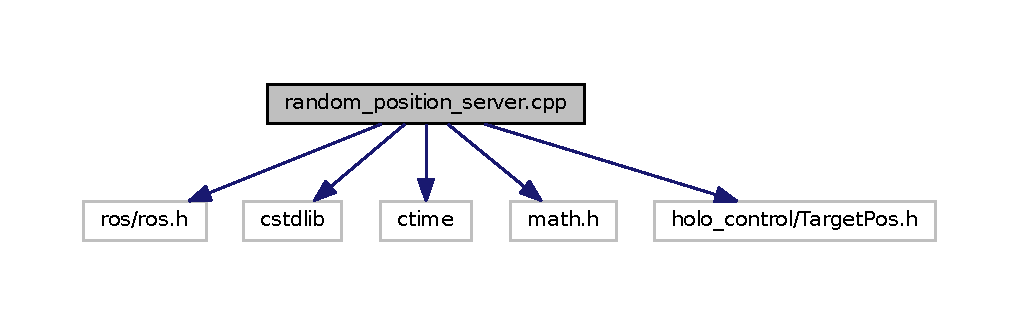
\includegraphics[width=350pt]{random__position__server_8cpp__incl}
\end{center}
\end{figure}
\subsection*{Functions}
\begin{DoxyCompactItemize}
\item 
bool \hyperlink{random__position__server_8cpp_aa87fa309f7fd2e88fd4091f304ed3a47}{rand\+\_\+pos} (holo\+\_\+control\+::\+Target\+Pos\+::\+Request \&req, holo\+\_\+control\+::\+Target\+Pos\+::\+Response \&res)
\item 
int \hyperlink{random__position__server_8cpp_a0ddf1224851353fc92bfbff6f499fa97}{main} (int argc, char $\ast$argv\mbox{[}$\,$\mbox{]})
\end{DoxyCompactItemize}


\subsection{Function Documentation}
\index{random\+\_\+position\+\_\+server.\+cpp@{random\+\_\+position\+\_\+server.\+cpp}!main@{main}}
\index{main@{main}!random\+\_\+position\+\_\+server.\+cpp@{random\+\_\+position\+\_\+server.\+cpp}}
\subsubsection[{\texorpdfstring{main(int argc, char $\ast$argv[])}{main(int argc, char *argv[])}}]{\setlength{\rightskip}{0pt plus 5cm}int main (
\begin{DoxyParamCaption}
\item[{int}]{argc, }
\item[{char $\ast$}]{argv\mbox{[}$\,$\mbox{]}}
\end{DoxyParamCaption}
)}\hypertarget{random__position__server_8cpp_a0ddf1224851353fc92bfbff6f499fa97}{}\label{random__position__server_8cpp_a0ddf1224851353fc92bfbff6f499fa97}


Definition at line 38 of file random\+\_\+position\+\_\+server.\+cpp.

\index{random\+\_\+position\+\_\+server.\+cpp@{random\+\_\+position\+\_\+server.\+cpp}!rand\+\_\+pos@{rand\+\_\+pos}}
\index{rand\+\_\+pos@{rand\+\_\+pos}!random\+\_\+position\+\_\+server.\+cpp@{random\+\_\+position\+\_\+server.\+cpp}}
\subsubsection[{\texorpdfstring{rand\+\_\+pos(holo\+\_\+control\+::\+Target\+Pos\+::\+Request \&req, holo\+\_\+control\+::\+Target\+Pos\+::\+Response \&res)}{rand_pos(holo_control::TargetPos::Request &req, holo_control::TargetPos::Response &res)}}]{\setlength{\rightskip}{0pt plus 5cm}bool rand\+\_\+pos (
\begin{DoxyParamCaption}
\item[{holo\+\_\+control\+::\+Target\+Pos\+::\+Request \&}]{req, }
\item[{holo\+\_\+control\+::\+Target\+Pos\+::\+Response \&}]{res}
\end{DoxyParamCaption}
)}\hypertarget{random__position__server_8cpp_aa87fa309f7fd2e88fd4091f304ed3a47}{}\label{random__position__server_8cpp_aa87fa309f7fd2e88fd4091f304ed3a47}
Server response returning two random values

This function inserts two random values between -\/6.\+0 and 6.\+0 each inside the response field of a service.


\begin{DoxyParams}{Parameters}
{\em req} & (holo\+\_\+control\+::\+Target\+Pos\+::\+Request \&)\+: request field of the Target\+Pos service of package holo\+\_\+control, not utilized (being it acutally empty); \\
\hline
{\em res} & (holo\+\_\+control\+::\+Target\+Pos\+::\+Response \&)\+: response field of the Target\+Pos service of package holo\+\_\+control, is a Point (defined in \char`\"{}geometry\+\_\+msgs\char`\"{}) named \textquotesingle{}target\+\_\+pos\textquotesingle{} its fields x and y are set to a float random value between -\/6.\+0 and 6.\+0;\\
\hline
\end{DoxyParams}

\begin{DoxyRetVals}{Return values}
{\em flag} & (bool)\+: flag unused, set to \textquotesingle{}true\textquotesingle{}; \\
\hline
\end{DoxyRetVals}


Definition at line 32 of file random\+\_\+position\+\_\+server.\+cpp.


\hypertarget{target__velocity__server_8cpp}{}\section{target\+\_\+velocity\+\_\+server.\+cpp File Reference}
\label{target__velocity__server_8cpp}\index{target\+\_\+velocity\+\_\+server.\+cpp@{target\+\_\+velocity\+\_\+server.\+cpp}}
{\ttfamily \#include \char`\"{}ros/ros.\+h\char`\"{}}\\*
{\ttfamily \#include \char`\"{}geometry\+\_\+msgs/\+Twist.\+h\char`\"{}}\\*
{\ttfamily \#include \char`\"{}nav\+\_\+msgs/\+Odometry.\+h\char`\"{}}\\*
{\ttfamily \#include \char`\"{}holo\+\_\+control/\+Target\+Vel.\+h\char`\"{}}\\*
Include dependency graph for target\+\_\+velocity\+\_\+server.\+cpp\+:\nopagebreak
\begin{figure}[H]
\begin{center}
\leavevmode
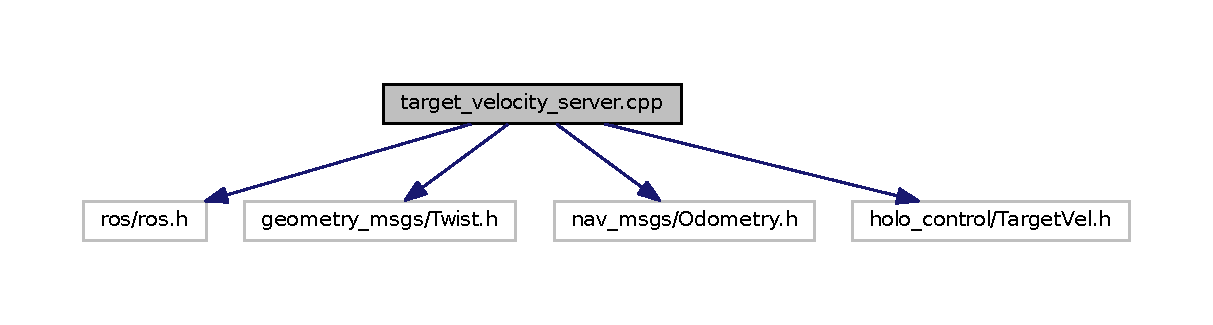
\includegraphics[width=350pt]{target__velocity__server_8cpp__incl}
\end{center}
\end{figure}
\subsection*{Functions}
\begin{DoxyCompactItemize}
\item 
void \hyperlink{target__velocity__server_8cpp_aef70658f8ec02213922917e67d9e1c76}{subscriber\+Callback} (const nav\+\_\+msgs\+::\+Odometry\+::\+Const\+Ptr \&pose\+\_\+msg)
\item 
bool \hyperlink{target__velocity__server_8cpp_a36957a375fbd4b38b8711d9aeeff44d3}{target\+\_\+vel} (holo\+\_\+control\+::\+Target\+Vel\+::\+Request \&req, holo\+\_\+control\+::\+Target\+Vel\+::\+Response \&res)
\item 
int \hyperlink{target__velocity__server_8cpp_a0ddf1224851353fc92bfbff6f499fa97}{main} (int argc, char $\ast$argv\mbox{[}$\,$\mbox{]})
\end{DoxyCompactItemize}
\subsection*{Variables}
\begin{DoxyCompactItemize}
\item 
geometry\+\_\+msgs\+::\+Twist \hyperlink{target__velocity__server_8cpp_ae43153a40663df7e24fce570690fff81}{current\+\_\+vel}
\item 
int \hyperlink{target__velocity__server_8cpp_ab66ed8e0098c0a86b458672a55a9cca9}{k} = 1
\item 
float \hyperlink{target__velocity__server_8cpp_a5bf563dfc55db9dac98ac73ed7a8df92}{alfa} = 0.\+1
\end{DoxyCompactItemize}


\subsection{Function Documentation}
\index{target\+\_\+velocity\+\_\+server.\+cpp@{target\+\_\+velocity\+\_\+server.\+cpp}!main@{main}}
\index{main@{main}!target\+\_\+velocity\+\_\+server.\+cpp@{target\+\_\+velocity\+\_\+server.\+cpp}}
\subsubsection[{\texorpdfstring{main(int argc, char $\ast$argv[])}{main(int argc, char *argv[])}}]{\setlength{\rightskip}{0pt plus 5cm}int main (
\begin{DoxyParamCaption}
\item[{int}]{argc, }
\item[{char $\ast$}]{argv\mbox{[}$\,$\mbox{]}}
\end{DoxyParamCaption}
)}\hypertarget{target__velocity__server_8cpp_a0ddf1224851353fc92bfbff6f499fa97}{}\label{target__velocity__server_8cpp_a0ddf1224851353fc92bfbff6f499fa97}


Definition at line 97 of file target\+\_\+velocity\+\_\+server.\+cpp.

\index{target\+\_\+velocity\+\_\+server.\+cpp@{target\+\_\+velocity\+\_\+server.\+cpp}!subscriber\+Callback@{subscriber\+Callback}}
\index{subscriber\+Callback@{subscriber\+Callback}!target\+\_\+velocity\+\_\+server.\+cpp@{target\+\_\+velocity\+\_\+server.\+cpp}}
\subsubsection[{\texorpdfstring{subscriber\+Callback(const nav\+\_\+msgs\+::\+Odometry\+::\+Const\+Ptr \&pose\+\_\+msg)}{subscriberCallback(const nav_msgs::Odometry::ConstPtr &pose_msg)}}]{\setlength{\rightskip}{0pt plus 5cm}void subscriber\+Callback (
\begin{DoxyParamCaption}
\item[{const nav\+\_\+msgs\+::\+Odometry\+::\+Const\+Ptr \&}]{pose\+\_\+msg}
\end{DoxyParamCaption}
)}\hypertarget{target__velocity__server_8cpp_aef70658f8ec02213922917e67d9e1c76}{}\label{target__velocity__server_8cpp_aef70658f8ec02213922917e67d9e1c76}
Callback reading current estimated velocity and saving it for retrieval by the Service call

This function updates the values saved inside the global variable \textquotesingle{}current\+\_\+vel\textquotesingle{} each time a new state estimation is published on the topic \char`\"{}/odom\char`\"{}


\begin{DoxyParams}{Parameters}
{\em pose\+\_\+msg} & (const nav\+\_\+msgs\+::\+Odometry\+::\+Const\+Ptr\&)\+: the current estimated state of the robot, as published in the topic \char`\"{}/odom\char`\"{} \\
\hline
\end{DoxyParams}


Definition at line 29 of file target\+\_\+velocity\+\_\+server.\+cpp.

\index{target\+\_\+velocity\+\_\+server.\+cpp@{target\+\_\+velocity\+\_\+server.\+cpp}!target\+\_\+vel@{target\+\_\+vel}}
\index{target\+\_\+vel@{target\+\_\+vel}!target\+\_\+velocity\+\_\+server.\+cpp@{target\+\_\+velocity\+\_\+server.\+cpp}}
\subsubsection[{\texorpdfstring{target\+\_\+vel(holo\+\_\+control\+::\+Target\+Vel\+::\+Request \&req, holo\+\_\+control\+::\+Target\+Vel\+::\+Response \&res)}{target_vel(holo_control::TargetVel::Request &req, holo_control::TargetVel::Response &res)}}]{\setlength{\rightskip}{0pt plus 5cm}bool target\+\_\+vel (
\begin{DoxyParamCaption}
\item[{holo\+\_\+control\+::\+Target\+Vel\+::\+Request \&}]{req, }
\item[{holo\+\_\+control\+::\+Target\+Vel\+::\+Response \&}]{res}
\end{DoxyParamCaption}
)}\hypertarget{target__velocity__server_8cpp_a36957a375fbd4b38b8711d9aeeff44d3}{}\label{target__velocity__server_8cpp_a36957a375fbd4b38b8711d9aeeff44d3}
Server response returning target velocity

Each time a call request is made to the Service \char`\"{}/\+Target\+Vel\char`\"{} a velocity value is computed based on the current and target point coordinates, passed in the request field of the Service, and on a \char`\"{}target\+\_\+mode\char`\"{} defining which of the implemented algorithm to use for the computation. Currently two such algorithms are implemented\+:~\newline

\begin{DoxyItemize}
\item 0\+: velocity is directly proportional to current distance from target position;~\newline

\item 1\+: velocity is the weighted sum between one component being being proportional to current distance from target position, and the previous velocity;
\end{DoxyItemize}


\begin{DoxyParams}{Parameters}
{\em req} & (holo\+\_\+control\+::\+Target\+Vel\+::\+Request \&)\+: request field of the Target\+Vel service of package holo\+\_\+control, composed of two Point(s) called \textquotesingle{}current\+\_\+pos\textquotesingle{} and \textquotesingle{}target\+\_\+pos\textquotesingle{} and one integer called \textquotesingle{}target\+\_\+mode\textquotesingle{}; \\
\hline
{\em res} & (holo\+\_\+control\+::\+Target\+Pos\+::\+Response \&)\+: response field of the Target\+Vel service of package holo\+\_\+control, is a Twist (defined in \char`\"{}geometry\+\_\+msgs\char`\"{}) named \textquotesingle{}twist\textquotesingle{} \\
\hline
\end{DoxyParams}

\begin{DoxyRetVals}{Return values}
{\em flag} & (bool)\+: flag unused, set to \textquotesingle{}true\textquotesingle{}; \\
\hline
\end{DoxyRetVals}


Definition at line 66 of file target\+\_\+velocity\+\_\+server.\+cpp.



\subsection{Variable Documentation}
\index{target\+\_\+velocity\+\_\+server.\+cpp@{target\+\_\+velocity\+\_\+server.\+cpp}!alfa@{alfa}}
\index{alfa@{alfa}!target\+\_\+velocity\+\_\+server.\+cpp@{target\+\_\+velocity\+\_\+server.\+cpp}}
\subsubsection[{\texorpdfstring{alfa}{alfa}}]{\setlength{\rightskip}{0pt plus 5cm}float alfa = 0.\+1}\hypertarget{target__velocity__server_8cpp_a5bf563dfc55db9dac98ac73ed7a8df92}{}\label{target__velocity__server_8cpp_a5bf563dfc55db9dac98ac73ed7a8df92}
Weight in the sum in case the mode of the service is set to 1, simulating inertia 

Definition at line 10 of file target\+\_\+velocity\+\_\+server.\+cpp.

\index{target\+\_\+velocity\+\_\+server.\+cpp@{target\+\_\+velocity\+\_\+server.\+cpp}!current\+\_\+vel@{current\+\_\+vel}}
\index{current\+\_\+vel@{current\+\_\+vel}!target\+\_\+velocity\+\_\+server.\+cpp@{target\+\_\+velocity\+\_\+server.\+cpp}}
\subsubsection[{\texorpdfstring{current\+\_\+vel}{current_vel}}]{\setlength{\rightskip}{0pt plus 5cm}geometry\+\_\+msgs\+::\+Twist current\+\_\+vel}\hypertarget{target__velocity__server_8cpp_ae43153a40663df7e24fce570690fff81}{}\label{target__velocity__server_8cpp_ae43153a40663df7e24fce570690fff81}
Twist used to contain the current estimated value of the robot velocities 

Definition at line 7 of file target\+\_\+velocity\+\_\+server.\+cpp.

\index{target\+\_\+velocity\+\_\+server.\+cpp@{target\+\_\+velocity\+\_\+server.\+cpp}!k@{k}}
\index{k@{k}!target\+\_\+velocity\+\_\+server.\+cpp@{target\+\_\+velocity\+\_\+server.\+cpp}}
\subsubsection[{\texorpdfstring{k}{k}}]{\setlength{\rightskip}{0pt plus 5cm}int k = 1}\hypertarget{target__velocity__server_8cpp_ab66ed8e0098c0a86b458672a55a9cca9}{}\label{target__velocity__server_8cpp_ab66ed8e0098c0a86b458672a55a9cca9}
Coefficient used in the linear computation of instantaneous velocity 

Definition at line 9 of file target\+\_\+velocity\+\_\+server.\+cpp.


%--- End generated contents ---

% Index
\backmatter
\newpage
\phantomsection
\clearemptydoublepage
\addcontentsline{toc}{chapter}{Index}
\printindex

\end{document}
